\documentclass{article}
\usepackage{amsmath, amssymb, graphicx, hyperref, geometry, float}

\geometry{top=1in, bottom=1in, left=1in, right=1in}

\title{Nonlinear ODEs and Linear PDEs Equivalence in Fluid Dynamics}
\author{By: Romerico David}
\date{}
\begin{document}

\maketitle

\begin{center}
\section*{Author of the Research Paper:}
John D. Ramshaw\\
Department of Physics, Portland State University, Portland, Oregon 97207
\end{center}

\section*{Other Contributors}
\begin{enumerate}
    \item Micah Lawal
    \item James Minter
    \item Mauro Sgromo
\end{enumerate}



\section{Introduction}

\subsection{Problem Statement}
Exploring the relations between nonlinear ordinary differential equations (ODEs) and linear partial differential equations (PDEs) within the context of fluid dynamics. This topic is not widely taught and is often undervalued.

\subsection{Solution Method}
Construct solutions to certain PDEs occurring in fluid dynamics by using the equivalence between nonlinear ODEs and linear PDEs. Specifically, this involves expressing the solutions to PDEs in terms of the solutions to corresponding ODEs.

\section{Assumptions}
\begin{enumerate}
    \item The fluid velocity field, $\mathbf{u}(\mathbf{x}, t)$, is known or can be determined.
    \item The fluid velocity fields are relatively simple.
    \item The scalar quantities being advected are non-diffusive.
    \item The fluid motion can be described using Lagrangian surfaces.
\end{enumerate}

\section{Unfamiliar Terms}
\begin{itemize}
    \item \textbf{Advection:} The movement of a mass/particle because of the fluid.
    \item \textbf{Non-Diffusive Scalar:} A scalar quantity that remains constant for individual fluid particles as they move through the fluid.
    \item \textbf{Lagrangian Surface:} A surface that moves with the velocity field and the points on the surface stay in the same orientation.
    \item \textbf{Lagrangian Trajectory:} The path a fluid particle follows as it moves through space and time.
\end{itemize}

\section{Lagrangian Trajectories}
Lagrangian Trajectories describe the paths of fluid particles as they move through the fluid via differential equations.

\subsection{Key Concept}
The focus is on following individual particles rather than looking at specific locations in space (Eulerian approach).

\subsection{Key Equations}
\begin{itemize}
    \item Position vector of a Lagrangian fluid particle $\mathbf{x}$ is governed by the nonlinear ODE $\dot{\mathbf{x}} = \mathbf{u}(\mathbf{x}, t)$ where $\mathbf{u}(\mathbf{x}, t)$ is the velocity field.
    \item Solution $\mathbf{x} = F(t, \mathbf{X})$ with $\mathbf{X}$ as the initial position.
    \item Reverse transformation: $\mathbf{X} = G(t, \mathbf{x})$.
\end{itemize}

\subsection{Transformations}
\begin{itemize}
    \item From Eulerian to Lagrangian coordinates: Defined by $\mathbf{X} = G(t, \mathbf{x})$
    \item Reverse process: Defined by $\mathbf{x} = F(t, \mathbf{X})$
\end{itemize}
Differentiating $\mathbf{X} = G(t, \mathbf{x})$ with respect to time:
\begin{equation}
\frac{\partial \mathbf{X}}{\partial t} = \frac{\partial G(t,\mathbf{x})}{\partial t} + \frac{\partial G(t,\mathbf{x})}{\partial \mathbf{x}} \cdot \frac{\partial \mathbf{x}}{\partial t}
\end{equation}
Since $\mathbf{X}$ is constant:
\begin{equation}
0 = \frac{\partial G(t,\mathbf{x})}{\partial t} + \mathbf{u}(\mathbf{x},t) \cdot \nabla G(t, \mathbf{x})
\end{equation}
This results in the first-order linear PDE:
\begin{equation}
\frac{\partial G}{\partial t} + \mathbf{u} \cdot \nabla G = 0
\end{equation}
which shows how transformations related to fluid particle trajectories adhere to linear dynamics even though the original ODE is nonlinear.

\begin{figure}[H]
    \centering
    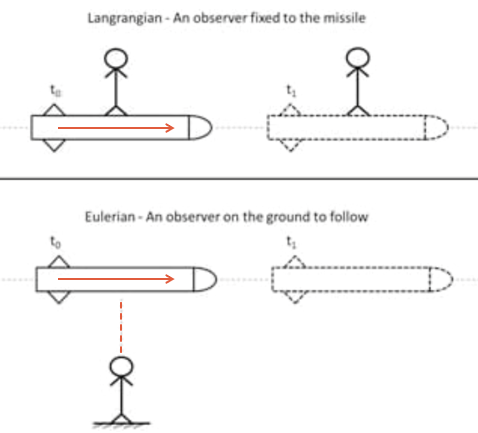
\includegraphics[width=0.5\textwidth]{./src/figures/lagrangian_vs_eulerian.PNG} 
    \caption{
        Lagrangian vs. Eulerian\\
        \textbf{Lagrangian:} Focuses on tracking individual fluid particles over time.\\
        \textbf{Eulerian:} Focuses on how fluid properties change at specific locations in space over time.
    }
    \label{fig:lagrangian_vs_eulerian}
\end{figure}

\section{Understanding the Non-Diffusive Scalar}

\subsection{Definition}
A non-diffusive scalar $f(\mathbf{x}, t)$ in fluid dynamics is a scalar quantity that remains constant along the trajectory of any fluid particle.

\subsection{Explanation}
Following the equation for $\mathbf{x}$:
\begin{equation}
f(\mathbf{x}, t) = f_0(\mathbf{X}) \quad \text{where} \quad \mathbf{X} \text{ is the initial position of the particle}
\end{equation}
which transforms to the exact general solution:
\begin{equation}
f(\mathbf{x}, t) = f_0(G(t, \mathbf{x}))
\end{equation}
from the initial condition $\mathbf{X} = G(t, \mathbf{x})$.

\subsection{Using the Method of Characteristics}
Additionally, when we solve the PDE
\begin{equation}
\frac{\partial f}{\partial t} + \mathbf{u} \cdot \nabla f = 0
\end{equation}
using the method of characteristics will result in a system of characteristic equations that will give us the same exact general solution under the same initial conditions
\begin{equation}
f(\mathbf{x}, t) = f_0(G(t, \mathbf{x}))
\end{equation}

\section{Method of Characteristics}

\subsection{Example using Method of Characteristics}
Consider the first-order linear PDE:
\begin{equation}
a(x, t)u_x + b(x, t)u_t = c(x, t)
\end{equation}
Dropping arguments:
\begin{equation}
a u_x + b u_t - c = 0
\end{equation}
By the definition of a directional derivative:
\begin{equation}
D_u f(x, t) = f_x \cdot a + f_t \cdot b
\end{equation}
and dot product of vectors \( \mathbf{v} \) and \( \mathbf{u} \) (arbitrary):
\begin{equation}
\mathbf{v} \cdot \mathbf{u} = v_1 u_1 + v_2 u_2 + v_3 u_3
\end{equation}
We perform the reverse transformation:
\begin{equation}
a u_x + b u_t - c = \langle a, b, -c \rangle \cdot \langle u_x, u_t, -1 \rangle = 0
\end{equation}
If \( \langle a, b, -c \rangle \) is perpendicular (orthogonal) to \( \langle u_x, u_t, -1 \rangle \), \( \langle a, b, -c \rangle \) lies in the tangent plane to the surface \( S \) and we can construct a curve \( C \) parametrized by \( s \) such that at each point on \( C \), the vector \( \langle a(x, t), b(x, t), c(x, t) \rangle \) is tangent to the curve.

\subsection{Parametrization along \(s\)}
Parametrization along \(s\) is called characteristic curves:
\begin{equation}
C = \{x = x(s), t = t(s), z = z(s)\}
\end{equation}
Following the chain rule:
\begin{equation}
\frac{d}{ds} = \frac{\partial}{\partial x} \frac{dx}{ds} + \frac{\partial}{\partial t} \frac{dt}{ds} = u_x a + u_t b = c
\end{equation}
Matching coefficients:
\begin{equation}
\frac{dx}{ds} = a(x, t), \quad \frac{dt}{ds} = b(x, t), \quad \frac{du}{ds} = c(x, t)
\end{equation}
Thus we have the set of characteristic equations given as:
\begin{equation}
\frac{dx}{ds} = a(x(s), t(s)), \quad \frac{dt}{ds} = b(x(s), t(s)), \quad \frac{du}{ds} = c(x(s), t(s))
\end{equation}
Our linear PDE was reduced into a system of ODEs where we can use our knowledge of ODEs to solve the characteristic equations.

\section{Lagrangian Surfaces in Fluid Dynamics}
A Lagrangian surface \( S(t) \) is a collection of fluid particles that move with the fluid velocity field \( \mathbf{u}(\mathbf{x}, t) \) to form a coherent surface.

\subsection{Definition and Parameterization}
The initial surface \( S(0) \) can be parameterized by a function \( Q_0(\alpha, \beta) \) defined by:
\begin{equation}
\mathbf{X} = Q_0(\alpha, \beta)
\end{equation}
where \( (\alpha, \beta) \) are parameters that uniquely identify points on the initial surface.
The Lagrangian surface at a later time \( t \) can be defined by:
\begin{equation}
\mathbf{x} = Q(t, \alpha, \beta) \quad \text{where} \quad Q(t, \alpha, \beta) = F(t, Q_0(\alpha, \beta))
\end{equation}

\section{Example: Incompressible Spherically Symmetric Radial Velocity Field in Spherical Coordinates}
\subsection{Solving the PDE}
Given the velocity field:
\begin{equation}
\mathbf{u} = u(r, t) \mathbf{e}_r
\end{equation}
where \(\mathbf{e}_r\) is the radial unit vector. 
The advection equation in spherical coordinates for an incompressible fluid is given by:
\begin{equation}
\frac{1}{r^2} \frac{\partial}{\partial r} (r^2 u) = 0
\end{equation}
Integrating this equation:
\begin{equation}
r^2 u = a(t) \quad \Rightarrow \quad u(r, t) = \frac{a(t)}{r^2}
\end{equation}
The position vector \(\mathbf{x}\) in spherical coordinates is given as:
\begin{equation}
\mathbf{x} = r \mathbf{e}_r
\end{equation}
Differentiating with respect to time:
\begin{equation}
\dot{\mathbf{x}} = \frac{d}{dt} (r \mathbf{e}_r) = \dot{r} \mathbf{e}_r + r \dot{\mathbf{e}}_r = \frac{a(t)}{r^2} \mathbf{e}_r
\end{equation}
Using the identity \( \mathbf{e}_r \cdot \mathbf{e}_r = 1 \Rightarrow \dot{\mathbf{e}}_r \cdot \mathbf{e}_r = 0 \), which means that \(\dot{\mathbf{e}}_r\) is orthogonal to \(\mathbf{e}_r\), thus it does not contribute to the radial component.

\(a(t)\) can be eliminated in terms of the time dependence by using a particular reference Lagrangian radius \(R(t)\) satisfying our radial velocity. This means we can define \(r = R(t)\) as the radius of the unperturbed interface, which is the boundary between the particle and surface but remains unaffected by other variables since the surface is a nearly spherical interface, thus its geometry cancels opposing inertial forces.

Thus, 
\[\dot{R} = \frac{a(t)}{R^2} \implies a(t) = R^2 \dot{R}\]

So,
\[\dot{r} = \frac{R^2 \dot{R}}{r^2}\]

Assuming \(r(0) = r_0\) and \(R(0) = R_0\):
\[r^2 \dot{r} = R^2 \dot{R}\]

Integrating both sides:
\[\int_{r_0}^{r} r^2 dr = \int_{R_0}^{R} R^2 dR\]

We get:
\[ r = \left[ R^3(t) - R_0^3 + r_0^3 \right]^{\frac{1}{3}} \]
or
\[ r_0 = \left[ R^3(t) - R_0^3 + r^3 \right]^{\frac{1}{3}} \]

where \(r_0\) is the radial coordinate of \(X\).

According to our non-diffusive scalar function with the initial condition \(f_0(r_0, \theta, \phi)\) at \(t = 0\), the exact general solution is:
\begin{equation}
f(r, \theta, \phi, t) = f_0(R^3(t) - R^3(0) + r^3(0), \theta, \phi)
\end{equation}
Additionally, using the method of characteristics on the advection equation:
\begin{equation}
\frac{\partial f}{\partial t} + \mathbf{u} \cdot \nabla f = 0
\end{equation}
where \( \mathbf{u} = u(r, t) \mathbf{e}_r \), will result in a system of characteristic equations that also gives us our exact general solution:
\begin{equation}
f(r, \theta, \phi, t) = f_0 \left( \left( R(t)^3 - R_0^3 + r^3 \right)^{1/3}, \theta, \phi \right)
\end{equation}
with the initial condition \( f_0(r_0, \theta, \phi) \) at \( t = 0 \).

\subsection{Volume Conservation}
The surface is initially defined by \(r_0 = Q_0(\alpha, \beta)\) at \(t = 0\). The radius of the surface at a later time \(t\) is defined by:
\[
r = \left( R(t)^3 - R_0^3 + Q_0^3(\alpha, \beta) \right)^{1/3}
\]
This shows how the radius \(r\) evolves from its initial configuration through some Lagrangian deformation \(R(t)\). The aim is to ensure that the deformation from \(r_0\) to \(r\) preserves the volume enclosed by the surface, meaning every point on the initial surface retains its volume at later times.

Since both states are Lagrangian, if the initial condition is satisfied, then all later conditions will also be satisfied. So, we can define \(r_0\) by:
\begin{equation}
\frac{4\pi}{3} R_0^3 = \int_{0}^{2\pi} \int_{-\pi}^{\pi} \int_{0}^{Q_0} r^2 dr \sin\theta \, d\theta \, d\phi
\end{equation}

This can be simplified to:
\begin{equation}
\frac{4\pi}{3} R_0^3 = \int_{0}^{2\pi} \int_{-\pi}^{\pi} Q_0^3(\theta, \phi) \sin\theta \, d\theta \, d\phi
\end{equation}
\begin{equation}
= \frac{1}{3} \int_{0}^{2\pi} \int_{-\pi}^{\pi} Q_0^3(\theta, \phi) \sin\theta \, d\theta \, d\phi
\end{equation}

This step describes the mathematical formulation for how a deformable and spherically influenced fluid surface evolves over time while conserving its volume to set the stage for further analysis of such a system. In our simulation, we will only show how volume is conserved.

\section{Simulation}

\subsection{Using the Nonlinear ODE}
\begin{equation}
\dot{r} = \frac{a(t)}{r^2}
\end{equation}

We set \( a(t) = t \), a simple function of time, which results in:
\begin{equation}
\dot{r} = \frac{t}{r^2}
\end{equation}

\subsection{Simulation: Euler's Method}

The general formula for Euler's Method is:
\begin{equation}
r_{n+1} = r_n + h \cdot \dot{r}(t_n, r_n)
\end{equation}
where \( h \) is the time step and \( \dot{r}(t_n, r_n) = \frac{a(t)}{r_n^2} \).

Initial Conditions:
\begin{align*}
r_0 &= 1 \\
t_0 &= 0 \\
t_f &= 10 \\
h &= 0.01
\end{align*}

% \begin{figure}[H]
%     \centering
%     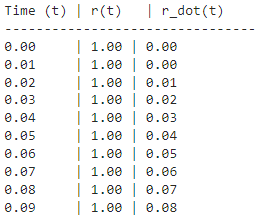
\includegraphics[width=0.4\textwidth]{euler_table.png} 
%     \caption{Simulation: Euler's Method Table Results}
%     \label{fig:euler_table}
% \end{figure}

\begin{figure}[H]
    \centering
    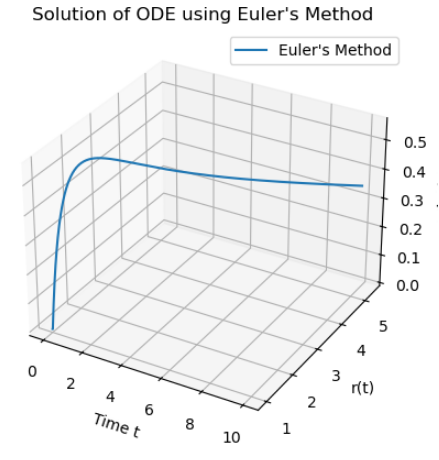
\includegraphics[width=0.5\textwidth]{./src/figures/euler_method_3d_plot.PNG} 
    \caption{Simulation: Euler's Method Graphical Plot in 3D and Table Results}
    \label{fig:euler_3d_plot}
\end{figure}

\begin{figure}[H]
    \centering
    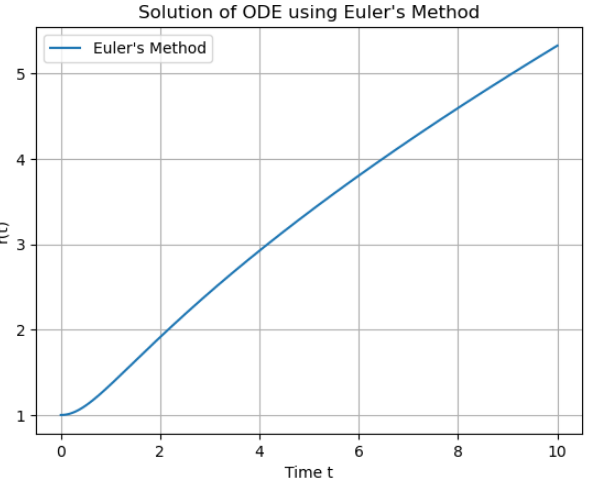
\includegraphics[width=0.5\textwidth]{./src/figures/euler_method_2d_plot.PNG} 
    \caption{Euler's Method Graphical Plot in 2D}
    \label{fig:euler_2d_plot}
\end{figure}

\subsection{Simulation using Runge-Kutta Method}
Runge-Kutta uses four intermediate steps to compute the next value of \(r\):
\begin{align}
k_1 &= h f(t_n, r_n) \\
k_2 &= h f\left(t_n + \frac{h}{2}, r_n + \frac{k_1}{2}\right) \\
k_3 &= h f\left(t_n + \frac{h}{2}, r_n + \frac{k_2}{2}\right) \\
k_4 &= h f(t_n + h, r_n + k_3)
\end{align}
The next value:
\begin{equation}
r_{n+1} = r_n + \frac{h}{6} (k_1 + 2k_2 + 2k_3 + k_4)
\end{equation}

Initial Conditions:
\begin{align*}
r_0 &= 1 \\
t_0 &= 0 \\
t_f &= 10 \\
h &= 0.01
\end{align*}

\begin{figure}[H]
    \centering
    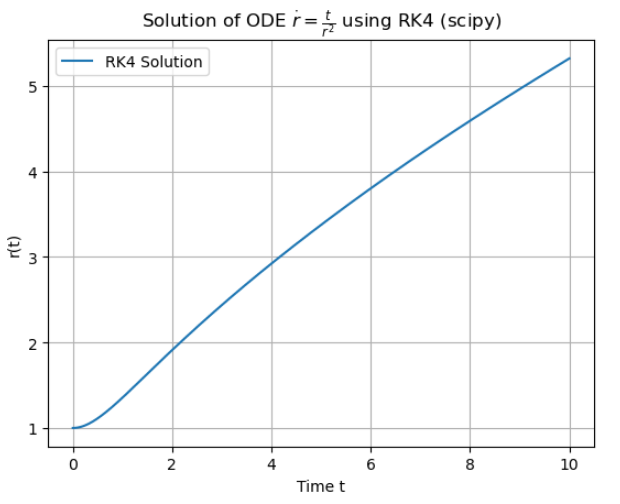
\includegraphics[width=0.5\textwidth]{./src/figures/runge_kutta_method.PNG} 
    \caption{Simulation: Runge-Kutta Method Graphical Plot in 2D}
    \label{fig:runge_kutta_2d_plot}
\end{figure}

\subsection{Results}

\textbf{Velocity Field:}
\begin{itemize}
    \item In spherical coordinates, our spherically symmetric radial velocity field \( \mathbf{u} = u(r, t)\mathbf{e}_r \) means that the velocity of fluid particles is directed radially outward and depends only on the radial distance \( r \) and time \( t \).
\end{itemize}

\textbf{Incompressibility:}
\begin{itemize}
    \item Incompressibility means the volume of any fluid element remains constant over time. This means volume is conserved if the deformation from \( r_0 \) to \( r \) remains constant.
\end{itemize}
Our simulations show that the radial displacement \(r\) steadily increases radially outward with time \(t\) under the influence of the velocity field. The deformation (slope) from initial radius \(r_0\) to any radius \(r\) remains constant, showing volume is conserved in our system. Given that the ODE \( \dot{r} = \frac{a(t)}{r^2} \) is equivalent to the PDE $\frac{1}{r^2} \frac{\partial}{\partial r} (r^2 u) = 0$, if we knew how to model a PDE, we expect similar results if we knew methods of modeling PDEs.

\subsection{New Variable: Adding Pressure and Viscosity}

We include the effects of pressure and viscosity in the radial component of the Navier-Stokes equations for an incompressible fluid. The general form of the Navier-Stokes equation for radial velocity \( u(r) \) in spherical coordinates, ignoring external forces like gravity for simplicity, is:

\begin{equation}
\rho \left( \frac{\partial u}{\partial t} + u \frac{\partial u}{\partial r} \right) = -\frac{\partial p}{\partial r} + \mu \left( \frac{\partial^2 u}{\partial r^2} + \frac{2}{r} \frac{\partial u}{\partial r} - \frac{2u}{r^2} \right)
\end{equation}

Let's assume that the velocity field \( u(r) = \frac{C}{r^2} \) is steady, so \( \frac{\partial u}{\partial t} = 0 \). Then compute the derivatives:
\begin{align}
\frac{\partial u}{\partial r} &= -\frac{2C}{r^3} \\
\frac{\partial^2 u}{\partial r^2} &= \frac{6C}{r^4}
\end{align}

Substituting these into the viscous term:
\begin{equation}
\mu \left( \frac{6C}{r^4} + \frac{2}{r} \left( -\frac{2C}{r^3} \right) - \frac{2C}{r^4} \right) = \mu \left( \frac{6C}{r^4} - \frac{4C}{r^4} - \frac{2C}{r^4} \right) = 0
\end{equation}

We can get a simplified equation:
\begin{equation}
-\frac{\partial p}{\partial r} = \rho \left( -\frac{2C^2}{r^5} \right)
\end{equation}

We then integrate the pressure gradient and are left with:
\begin{equation}
p(r) = -2\rho \frac{C^2}{3r^4} + p_0
\end{equation}

With \( C^2 \) determined by boundary conditions, such as specifying the velocity at a certain radius. The pressure varies inversely with the fourth power of the radius, illustrating how pressure gradients necessary to maintain such a flow increase sharply as \( r \) decreases.

This derivation encapsulates the interaction between the radial velocity profile and the pressure in a spherically symmetric, incompressible flow, showcasing the direct dependence of the pressure gradient on the square of the radial velocity field.

If we had more time, we would use this pressure equation added to our radial velocity to confirm whether the equivalence still holds true.

\section{References}
\begin{enumerate}
    \item Hautala, S. (2020). Advection-Diffusion Equation. In Physics Across Oceanography: Fluid Mechanics and Waves. University of Washington Pressbooks. Retrieved from \url{https://uw.pressbooks.pub/ocean285/chapter/advection-diffusion/}
    \item Pirola, A. (n.d.). Probability and Statistical Mechanics. Retrieved from \url{https://www.science.unitn.it/~pignatel/PoAV/talks/Pirola.pdf}
    \item Ramshaw, J. D. (2011). Nonlinear ordinary differential equations in fluid dynamics. \textit{American Journal of Physics}, 79(12), 1255-1260. Retrieved from \url{https://doi.org/10.1119/1.3636635}
    \item ScienceDirect Topics. (n.d.). Runge-Kutta Method. Retrieved from \url{https://www.sciencedirect.com/topics/mathematics/runge-kutta-method}
    \item Smyth, B. (n.d.). Lagrangian and Eulerian descriptions. In \textit{All Things Flow - Fluid Mechanics for the Natural Sciences}. LibreTexts. Retrieved from \url{https://eng.libretexts.org/Bookshelves/Civil_Engineering/Book\%3A_All_Things_Flow_-_Fluid_Mechanics_for_the_Natural_Sciences_(Smyth)/05\%3A_Fluid_Kinematics/5.01\%3A_Lagrangian_and_Eulerian_descriptions}
    \item Virtanen, P., et al. (2023). scipy.integrate.solve\_ivp [Documentation]. SciPy. Retrieved from \url{https://docs.scipy.org/doc/scipy/reference/generated/scipy.integrate.solve_ivp.html}
    \item YouTube. (2023). How to Solve PDEs and ODEs Using Euler's Method [Video]. YouTube. Retrieved from \url{https://www.youtube.com/watch?v=jdq6puyvQ7E&t=78s}
\end{enumerate}

\end{document}
